% Created 2019-10-15 Tue 19:26
% Intended LaTeX compiler: pdflatex
\documentclass[a4paper, sfsidenotes, justified, notitlepage]{tufte-book-lite}
     \input{/users/rakhim/.emacs.d/latex/tufte.tex}
\usepackage[utf8]{inputenc}
\usepackage[T1]{fontenc}
\usepackage{graphicx}
\usepackage{grffile}
\usepackage{longtable}
\usepackage{wrapfig}
\usepackage{rotating}
\usepackage[normalem]{ulem}
\usepackage{amsmath}
\usepackage{textcomp}
\usepackage{amssymb}
\usepackage{capt-of}
\usepackage{hyperref}
\author{Rakhim Davletkaliyev}
\date{\today}
\title{Computer Science For The Busy Developer}
\hypersetup{
 pdfauthor={Rakhim Davletkaliyev},
 pdftitle={Computer Science For The Busy Developer},
 pdfkeywords={},
 pdfsubject={},
 pdfcreator={Emacs 26.3 (Org mode 9.1.9)},
 pdflang={English}}
\begin{document}

\maketitle

\part{Intro}
\label{sec:orgd6f5f4f}

This course and the book constitute an high speed overview of the most important fundamental computer science areas. It is intended for intermediate and professional developers who, for any reason, are interested in getting to know the formal, academic side of CS better.

The goal is to provide an overview deep enough so that you end up understanding the ares, their problems and the connections between them. And shallow enough so that you aren't buried under hundreds of pages of proofs, formalizations and exercises.

We will start by trying to understand what computer science is and why it isn't a new area at all. We'll consider the computability as a fundamental property of reality rather than a technological apparatus.

We shall then proceed to learning essential mathematics necessary for further topics. These include proof techniques, notation and logic.

Next, we will learn about the following topics:

\marginnote{This is a margin note using the geometry package, set at 3cm vertical offset to the line it is typeseted.}

\begin{marginfigure}
  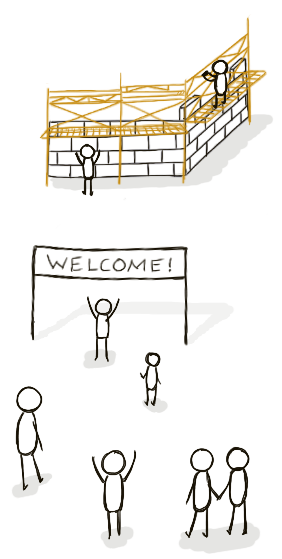
\includegraphics[width=\linewidth]{file}
  \caption{This is a margin figure}
  \label{fig:marginfig}
\end{marginfigure}

\begin{enumerate}
\item Algorithms. Complexity and examples of important algorithms in sorting.
\item Abstract Data Types.
\item Set theory.
\item Graph theory.
\item Theory of computation.
\item Cryptography.
\item Information theory.
\end{enumerate}

Since it seems impossible or at least unpractical to put all of computer science curriculum into a single course, even in a minified format, we shall leave the following topics for the last chapter. In it, we will give an overview to them:

\begin{itemize}
\item Abstract algebra
\item Category theory
\item Type theory
\item Computational geometry
\end{itemize}
\part{Foundations of Math}
\label{sec:orgcf00dc6}
\chapter{Set theory}
\label{sec:org59c5779}

\section{Intro to sets}
\label{sec:org119ed25}

Set theory is an important area of math which lays as a foundation of many computer science topics, such as databases, types in programming. Set theory isn't difficult conceptually, and is generally nice to think about, especially if you're a visual learner.

A set is simply a collection of things. A thing can be anything: name, object, idea. It's a very abstract notion.

For example, I can define a set of movies I have seen: American Pie, Breakfast Club, The Room. Yes, I have only seen those three movies in my entire life. I am busy writing computer science books.

Actually, I've watched The Room five times. Does this affect the set? No, because it doesn't change the notion of "what movies have I watched". This obvious thing is an integral property of sets: they include unique objects.

\marginnote{Nothing stops us from defining a set of movie viewings, though.}

If an object \(o\) is in set \(A\), we say \(o\) is a member of \(A\). To express this fact easily, mathematicians use the following notation: \(o \in A\).

So, if \(o\) is "The Room", and \(A\) is "Movies I've watched", then \(o \in A\). But if \(b\) is "Avengers", and I haven't watched Avengers, then \(b \notin A\).

If we were to look inside set \(A\), it might look like this:

\begin{equation}
\{s, m, o\}
\end{equation}



\begin{enumerate}
\item Ant hid?
\label{sec:orgb06ed79}

Since \(b \notin A\), we can't find \(b\) among the members.

Sets don't have the notion of order, so it doesn't matter how you mention its members as long as you mention them all. So, all these:

\begin{itemize}
\item \(\{s, m, o\}\)
\item \(\{s, o, m\}\)
\item \(\{m, s, o\}\)
\item etc.
\end{itemize}

describe the same set \(A\).


\begin{enumerate}
\item And even deeper?
\label{sec:org6d39605}

Here we were lucky: set \(A\) is finite and quite small. But sets can be infinite, and it would be impossible to write all its members. There are ways to describe such sets nevertheless. For example, the set of all natural numbers from 1 to n can be described like so:

\begin{equation}
\{1, 2, 3, 4, ... n\}
\end{equation}
\end{enumerate}
\end{enumerate}



\section{Empty set}
\label{sec:org1f25e64}

Mathematicians love zero. Ever since its inception around 1770 BC, zero is an important part of mathematical models. The notion of "nothingness", which zero reflects in the context of counting, is present in all areas. In the context of sets, nothingness is an \emph{empty set}.

Obviously, an empty set is a set without members.

\begin{equation}
\{\}
\end{equation}

Why would we need empty sets? Well, sometimes we want to describe a notion of having no objects under a certain description. For example, since I only watched 3 movies in my life, and all of them were American, I can describe a set of all non-American movies I've watched: it's an empty set \(Z = \{\}\).


\section{Subset, superset}
\label{sec:orgf825171}

When all members of set \(A\) are present in another set \(B\), then \(A\) is a subset of \(B\). This notion is expressed like so:

\begin{equation}
A \subseteq B
\end{equation}

Let's say set \(B\) is the set of all movies ever produced. Then \(A\) is clearly a subset of \(B\).

To look at things from the other end, \(B\) is a superset of \(A\):

\begin{equation}
B \supseteq A
\end{equation}

You know what else is a subset of \(B\)? An empty set!

\begin{equation}
\{\} \subseteq B
\end{equation}

This either sounds absolutely natural to you or extremely weird. This makes perfect sense to a mathematician, because it's easy to argue: \emph{all} members of \(\{\}\) are present in \(B\), all zero of them.

It gets weirder. As per our definition, if all members of a set are also present in another set, then the one is a subset of the other. This means any set is a subset of itself.

\begin{equation}
A \subseteq A \\
B \subseteq B \\
Z \subseteq B
\end{equation}

By extension, if two sets are the same, then any of them is a subset of the other.

Since often we only care about cases where sets aren't equal, there's a special notion of a \textbf{proper subset}.

If \(A\) is a subset of \(B\), but \(A\) is not equal to \(B\), then \(A\) is a proper subset of \(B\).

\begin{equation}
A \subset B
\end{equation}

So, a set if a subset of itself, but is never a proper subset of itself.
\end{document}
